\documentclass[tikz,border=8pt]{standalone}
% Shared look for every TikZ diagram. Load with % Shared look for every TikZ diagram. Load with % Shared look for every TikZ diagram. Load with \input{../../tools/tikz-style.tex}
\usepackage[T1]{fontenc}
\usepackage{lmodern}
\renewcommand{\sfdefault}{lmr}  % diagrams use the same serif as the text
\usetikzlibrary{arrows.meta, positioning, shapes.geometric, calc, fit, backgrounds}
\definecolor{cblue}{HTML}{4C78A8}
\definecolor{corange}{HTML}{F58518}
\definecolor{cgreen}{HTML}{54A24B}
\definecolor{cred}{HTML}{E45756}
\definecolor{cpurple}{HTML}{B279A2}
\definecolor{cgrey}{HTML}{6B6B6B}
\tikzset{
  every picture/.style={font=\sffamily, line width=1.2pt},
  box/.style={draw=#1, fill=#1!12, rounded corners=4pt, align=center, inner sep=7pt, minimum height=1.1cm},
  box/.default=cgrey,
  arrow/.style={-{Stealth[length=3mm]}, draw=cgrey, line width=1.4pt},
  title/.style={font=\sffamily\bfseries\Large},
  note/.style={font=\sffamily\small, text=cgrey, align=center},
}
\AtBeginDocument{\hyphenpenalty=10000 \exhyphenpenalty=10000}

\usepackage[T1]{fontenc}
\usepackage{lmodern}
\renewcommand{\sfdefault}{lmr}  % diagrams use the same serif as the text
\usetikzlibrary{arrows.meta, positioning, shapes.geometric, calc, fit, backgrounds}
\definecolor{cblue}{HTML}{4C78A8}
\definecolor{corange}{HTML}{F58518}
\definecolor{cgreen}{HTML}{54A24B}
\definecolor{cred}{HTML}{E45756}
\definecolor{cpurple}{HTML}{B279A2}
\definecolor{cgrey}{HTML}{6B6B6B}
\tikzset{
  every picture/.style={font=\sffamily, line width=1.2pt},
  box/.style={draw=#1, fill=#1!12, rounded corners=4pt, align=center, inner sep=7pt, minimum height=1.1cm},
  box/.default=cgrey,
  arrow/.style={-{Stealth[length=3mm]}, draw=cgrey, line width=1.4pt},
  title/.style={font=\sffamily\bfseries\Large},
  note/.style={font=\sffamily\small, text=cgrey, align=center},
}
\AtBeginDocument{\hyphenpenalty=10000 \exhyphenpenalty=10000}

\usepackage[T1]{fontenc}
\usepackage{lmodern}
\renewcommand{\sfdefault}{lmr}  % diagrams use the same serif as the text
\usetikzlibrary{arrows.meta, positioning, shapes.geometric, calc, fit, backgrounds}
\definecolor{cblue}{HTML}{4C78A8}
\definecolor{corange}{HTML}{F58518}
\definecolor{cgreen}{HTML}{54A24B}
\definecolor{cred}{HTML}{E45756}
\definecolor{cpurple}{HTML}{B279A2}
\definecolor{cgrey}{HTML}{6B6B6B}
\tikzset{
  every picture/.style={font=\sffamily, line width=1.2pt},
  box/.style={draw=#1, fill=#1!12, rounded corners=4pt, align=center, inner sep=7pt, minimum height=1.1cm},
  box/.default=cgrey,
  arrow/.style={-{Stealth[length=3mm]}, draw=cgrey, line width=1.4pt},
  title/.style={font=\sffamily\bfseries\Large},
  note/.style={font=\sffamily\small, text=cgrey, align=center},
}
\AtBeginDocument{\hyphenpenalty=10000 \exhyphenpenalty=10000}

\begin{document}
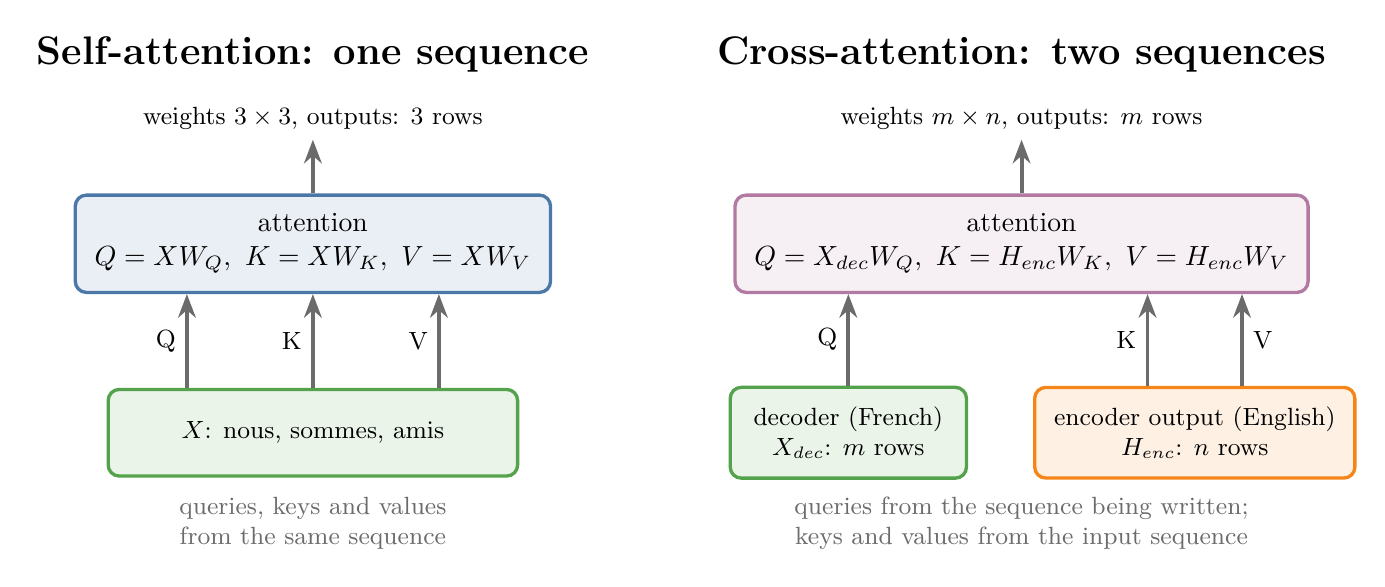
\begin{tikzpicture}[every node/.append style={font=\sffamily}]
  % ---------- self-attention ----------
  \node[title] at (2.6, 5.4) {Self-attention: one sequence};
  \node[box=cblue, minimum width=5.2cm] (sa) at (2.6, 3.0) {attention\\$Q = XW_Q,\ K = XW_K,\ V = XW_V$};
  \node[box=cgreen, minimum width=5.2cm, font=\small] (x) at (2.6, 0.6) {$X$: nous, sommes, amis};
  \foreach \dx/\l in {-1.6/Q, 0/K, 1.6/V}
    \draw[arrow] ([xshift=\dx cm]x.north) -- ([xshift=\dx cm]sa.south) node[midway, left, font=\small] {\l};
  \node[font=\small] (so) at (2.6, 4.6) {weights $3 \times 3$, outputs: 3 rows};
  \draw[arrow] (sa) -- (so);
  \node[note] at (2.6, -0.55) {queries, keys and values\\from the same sequence};
  % ---------- cross-attention ----------
  \node[title] at (11.6, 5.4) {Cross-attention: two sequences};
  \node[box=cpurple, minimum width=6.4cm] (ca) at (11.6, 3.0) {attention\\$Q = X_{dec}W_Q,\ K = H_{enc}W_K,\ V = H_{enc}W_V$};
  \node[box=cgreen, minimum width=3.0cm, font=\small, align=center] (dec) at (9.4, 0.6) {decoder (French)\\$X_{dec}$: $m$ rows};
  \node[box=corange, minimum width=3.0cm, font=\small, align=center] (enc) at (13.8, 0.6) {encoder output (English)\\$H_{enc}$: $n$ rows};
  \draw[arrow] (dec.north) -- (dec.north |- ca.south) node[midway, left, font=\small] {Q};
  \draw[arrow] ([xshift=-0.6cm]enc.north) -- ([xshift=-0.6cm]enc.north |- ca.south) node[midway, left, font=\small] {K};
  \draw[arrow] ([xshift=0.6cm]enc.north) -- ([xshift=0.6cm]enc.north |- ca.south) node[midway, right, font=\small] {V};
  \node[font=\small] (co) at (11.6, 4.6) {weights $m \times n$, outputs: $m$ rows};
  \draw[arrow] (ca) -- (co);
  \node[note] at (11.6, -0.55) {queries from the sequence being written;\\keys and values from the input sequence};
\end{tikzpicture}
\end{document}
